\documentclass[aps,pre,12pt,preprint,%
	onecolumn,showpacs,showkeys,nofootinbib]{revtex4-2}
%Chinese
	\usepackage[UTF8,fontset=fandol]{ctex}
%	\usepackage[datesep=/]{datetime2} % Use default
	\DeclareTextFontCommand{\textbf}{\sffamily}
%Presenting
	\usepackage[table]{xcolor}
	\usepackage{graphicx}
	\usepackage[font=small,format=plain,%
		labelfont=bf,textfont=it,%
		singlelinecheck=false]{caption}
	\usepackage[above]{placeins}
%	\usepackage{float} % Cause trouble for table footnotes
	\usepackage{wrapfig}
	\usepackage{tabularx,array,booktabs,multirow,bigstrut}
	\newcolumntype{C}[1]{>{\hsize=#1\hsize%
		\centering\arraybackslash}X}
	\newcommand{\minitab}[2][l]{%
		\begin{tabular}{#1}#2\end{tabular}}
	\usepackage{setspace,dcolumn}
	\usepackage{subfig}
	\usepackage{psfrag,epsfig}
%MathSetting
	\let\latexointop\ointop
	\usepackage{amsmath,bm,amssymb,esint,extarrows}
	\usepackage{upgreek,textcomp,mathrsfs}
	\usepackage[only,sslash]{stmaryrd}
	\usepackage{nicefrac,eqnarray}
%	\usepackage{amsthm} % Enable when necessary
%	\usepackage[mathscr]{eucal} % Enable when necessary
	\usepackage{mathtools,physics,siunitx}
	\usepackage{stackengine,varwidth}
	\usepackage{tikz}
	\usepackage{resizegather,empheq}
	\usetagform{default}
	\usepackage{calligra,fourier-orns}
	% Keep \oint unchanged by esint
	\let\ointop\undefined
	\let\ointop\latexointop
	% Define a scriptr 
	\DeclareMathAlphabet{\mathcalligra}{T1}{calligra}{m}{n}
	\DeclareFontShape{T1}{calligra}{m}{n}{<->s*[2.2]callig15}{}
	\newcommand{\scriptr}{\mathcalligra{r}\,}
	\newcommand{\rvector}{\pmb{\mathcalligra{r}}\,}
	% Useful shorthand
	\DeclarePairedDelimiter\ave{\langle}{\rangle}
	\newcommand\inlineeqno{\stepcounter{equation}\ (\theequation)}
	\newcommand{\sinc}{\operatorname{sinc}}
	\newcommand{\mbb}[1]{\mathbb{#1}}
	\newcommand{\mrm}[1]{\mathrm{#1}}
	\newcommand{\mcal}[1]{\mathcal{#1}}
	% Scaling and positioning
	\newcommand\scalemath[2]{\scalebox{#1}{\mbox{\ensuremath{\displaystyle #2}}}}
	\newcommand\raisemath[2]{\raisebox{#1\depth}{${#2}$}}
	\empheqset{box=\nicebox}
	% Presenting
	\newcommand*\nicebox[1]{\fbox{\hspace{1em}\addstackgap[5pt]{#1}\hspace{1em}}}

	\allowdisplaybreaks[2]
%ParagraphSetting
	\setlength{\parskip}{.3\baselineskip}
	\usepackage[defaultlines=2,all]{nowidow}
	\postdisplaypenalty=50
%PageSetting
	\usepackage{titlesec}
	\titleformat*{\section}{\large\bfseries}
	\usepackage[colorlinks=true,linkcolor=blue]{hyperref}
	\newcommand{\texstringonly}[1]{%
		\texorpdfstring{#1}{}}
	\usepackage[vmargin={3.5cm,4cm},hmargin=3cm,%
		footnotesep=\baselineskip]{geometry}
%	\usepackage[bottom]{footmisc} % Cause trouble for table footnotes
	\usepackage{changepage}
	% Autoref names
	\renewcommand{\tableautorefname}{\tablename}
	\renewcommand{\figureautorefname}{\figurename}
	% List settings
	\usepackage{enumitem}
	\setlist{itemsep=0pt,topsep=0pt,labelindent=\parindent,leftmargin=0pt,itemindent=*}
	% Some redefined lengths
	\setlength{\headsep}{1.6\baselineskip}
%	\setlength{\footnotesep}{3\parskip} % Use when necessary
	% Header
	\usepackage{fancyhdr,lastpage}
	\pagestyle{fancy}
%	\fancyhf{} % Clear default settings; disabled for now
	\cfoot{--\ \thepage\,/\,\pageref{LastPage} \ --}
	\setlength{\footskip}{2\baselineskip}
	\renewcommand{\headrulewidth}{0.1pt}
	\renewcommand{\headrule}{
		\ifnum\value{page}=1\relax\else
			\vbox to 2pt{
			\hbox to \headwidth{\dotfill}\vss}
		\fi}
	\fancypagestyle{titlepagestyle}{%
		\fancyhead{}
		\chead{
			\vspace{2.5\baselineskip}
			
\includegraphics[width=.75\linewidth]{../PKUPhy}}
	}
	% Separator
	\newcommand{\newparagraph}{\pagebreak[3]\noindent%
		\hfil
		~\raisebox{-4pt}[10pt][10pt]{\decofourright~~~~~~~~\decofourleft}~ %
		\par
	}
%	% Background % Use when necessary
%	\usepackage{background} %Waterstamp package
%	\SetBgContents{...的实验报告} %Waterstamp to prevent copying
%	\SetBgScale{5} %Waterstamp setting
	% Essay format
	\renewcommand\appendixname{附录}
	\renewcommand\abstractname{}
	\renewcommand\tablename{表}
	\renewcommand\figurename{图}
	\renewcommand\refname{参考文献}
	\renewcommand\contentsname{目录}
	\makeatletter
	\def\@pacs@name{\songti\zihao{-4}{\bf PACS码:}}
	\def\@keys@name{\songti\zihao{-4}{\bf 关键词:}}
	\def\Dated@name{日期:}
	\def\Received@name{\zihao{-5}{接收} }
	\def\Revised@name{\zihao{-5}{修订} }
	\def\Accepted@name{\zihao{-5}{采纳} }
	\def\Published@name{\zihao{-5}{发表} }
	\makeatother
	\linespread{1.5}
	\renewcommand{\labelenumi}{\alph{enumi}.}
	\leftmargini=20mm
	\newcommand{\supercite}[1]{\textsuperscript{\,%
		[\citenum{#1}]}}
	\let\fancycite\cite
	\renewcommand{\cite}[1]{\textup{\fancycite{#1}}}

%Miscellaneous
%	\newcommand{\tabindent}{\hspace{2em}}
%FourierTransform
	\newcommand{\fourierf}{\mathscr F}
\begin{document}
%Basic Data
	\title{%
	\texstringonly{\hfil\\[2\baselineskip]}
	\sf\LARGE%
		利用电子衍射分析晶体结构%
	\texstringonly{\vspace{3ex}}}
	\author{\fangsong\large%
		吴熙楠%
	\vspace{2mm}}
	\affiliation{\it%
		北京大学物理学院~~学号:\normalfont 1900011413\,}
	\date{\today}
	\keywords{电子衍射,波粒二象性,晶体结构,德拜环}
	\email{xinanwu@pku.edu.cn;}
	
\begin{abstract}
\vspace{10mm}
\begin{spacing}{1.5}\normalsize
\setlength{\parskip}{.3\baselineskip}
%	200—300字,
%	说明用什么方法做了什么事,
%	由此得到什么结果和结论,
%	有何意义. 
%	不用缩略词,不用第一人称.
%	
	本实验使用透射电子显微镜(Transmission electron microscope, TEM)获得电子经晶体散射的衍射图样,由此验证电子的波动特性;在此基础上,总结电子的衍射规律,并以此为工具分析晶体的结构。
	
	实验获得了金属多晶银、金、铜的衍射环(德拜环,Debye rings)以及单晶硅的衍射斑(劳厄斑,Laue spots),此现象强有力地验证了德布罗意的物质波假定;且以金为标准试样进行校准,借鉴衍射图样分析的一般方法,测定了其余样品的晶格常数。
\end{spacing}
\end{abstract}
\clearpage
\maketitle
\thispagestyle{titlepagestyle}
%
%	\item 课程实验报告应假定读者既不是已知全部实验细节的指导教师,也不是缺少专业知识的公众,而是同领域的实验研究者,或审稿人. 不能要求读者要在读过课程讲义后才能读懂课程实验报告.
%	\item 公式、图和表要分别用阿拉伯数字编列序号. 公式和图表要达到可发表的质量.
%	\item 凡不是自己独立思考得到的内容都应该引参考文献. 不能大段引用同一参考文献. 对复杂问题,应该优先考虑引用参考文献得到结果. 对简单一些的问题才鼓励独立思考.
%	\item 较长的推导和说明可以作为附件提交,不占用报告篇幅.
%	\item 思考题不是报告的组成部分. 应另起一页附在报告的最后.

\newpage
\section{引言}
%	研究论文引言一般包含以下内容:
%	(1)所研究领域背景和现状;
%	(2)有待研究的问题;
%	(3)本研究的目的、主要内容和结果;
%	(4)结果的意义.\par
%	在写实验报告的引言时,同学可以假想自己是第一个做类似研究的人.\par
%	引言一定要切合报告正文,不能漫无目的地介绍背景. 要快速地将读者引导到报告主题上,并作较深入的讨论.\par
%	引言篇幅可以在较大范围内变化,但最长不应超过报告文字篇幅的1/3.\par
%	引言撰写可以参考实验讲义,可以复述,但不能复制讲义上的任何一句话.\par
%%%%%%%%%%%%%%%%%%%%%%%%%%%%%%
	为了解决旧量子论中难以调和的诸多困难,1924年,德布罗意(Louis de Broglie)在其发表的博士论文 \cite{de1924recherches} 中提出了一种全新的量子化思路。德布罗意由爱因斯坦的光量子假定出发,推而广之,认为实物粒子同样具有波粒二象性,其\textit{相波}(phase wave)波长为:
	\begin{equation}
		\lambda = \frac{h}{p}
	\end{equation}
	该关系式与光量子的动量公式$p = \frac{h}{\lambda}$完全一致。对于电子而言,在非相对论情形下,$p = \sqrt{2mE} = \sqrt{2meU}$, 其中$U$为加速电压,则有:
	\begin{equation}
		\lambda \approxeq \sqrt{\frac{\SI{150}{\V}}{U}}\,\si{\angstrom}
		\label{eq:deBroglieLambda}
	\end{equation}
	
	这一假定的优越性在于,原先强加上的玻尔--索末菲量子化(Bohr-Sommerfeld quantization),即\textit{粒子的角动量(或系统的作用量)为$\hbar$(或$h$)的整数倍}这一条件,可由相波的\textit{共振条件}给出。所谓共振条件,指的是此时的相波为给定边界条件下的\textit{驻波}。对于原子而言,情况如 \autoref{fig:deBroglieOrbits} 所示。不难看出,这自然导致了量子化。
	\begin{figure}[!ht]
	\centering
	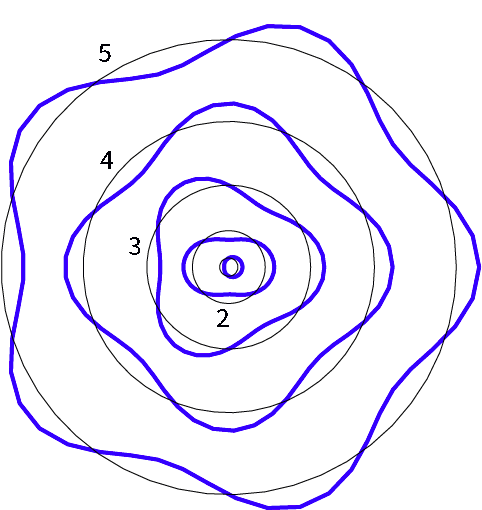
\includegraphics[width=.35\linewidth]{deBroglieOrbits.png}
	\caption[根据相波形成的驻波解释原子能级的量子化]{%
		根据相波形成的驻波解释原子能级的量子化%
		\vspace{3ex}
		\footnote{%
			图像据网络资源修改得到:\par
			\noindent\fontsize{9pt}{\parskip}%
			\url{https://skullsinthestars.com/2015/05/20/1975-the-year-that-quantum-mechanics-met-gravity/}}%
		}
	\label{fig:deBroglieOrbits}
	\end{figure}
	
	相波的假定暗示了实物粒子可像电磁波那样发生干涉和衍射。在相波观点的基础上,薛定谔(Erwin Schrödinger)于随后的两年内给出了相应的非相对论性波动方程:
	\begin{equation}
		i\hbar\,\pdv{\Psi}{t} = H\pqty{\vb{r},\vb{p},t}\,\Psi,\quad
		\vb{p} = -i\hbar\grad
	\end{equation}
	对于稳恒系统,例如原子的定态或恒定电子流的散射过程,可取$\Psi = \psi\,e^{-iEt/\hbar}$, 将问题简化为求解\textit{定态方程:}
	\begin{equation}
		H\pqty{\vb{r},\vb{p},t}\,\psi = E\psi
	\end{equation}
	
	利用这一方程,薛定谔给出了比玻尔模型更为精确、丰富的原子描述。特别地,对于$H = \frac{\vb{p}^2}{2m} + e\varphi(\vb{r})$, 方程展开为:
	\begin{equation}
		\laplacian{\psi}
			+ \frac{2m}{\hbar^2} \pqty{E - e\varphi}\,\psi = 0
	\end{equation}
	这是一个实的赫姆霍兹方程,完全类似于稳恒电磁波的传播;这进一步加强了前面的猜想,即特定能量的入射电子流可通过\textit{弹性散射}形成与电磁波散射完全类似的现象。果不其然,戴维森与革末(Clinton Davisson and Lester Germer)在以电子束轰击镍以研究其表面形貌时,意外地发现了电子在晶体表面反射形成的图样完全类似于X射线衍射图案\supercite{davisson1927diffraction};这便证实了物质波的假定。更进一步,X射线晶体学的相应方法均可推广至电子衍射,从而对衍射图样进行分析。
	
	在此基础上,如果样品充分地薄,使得电子流能够以充分的强度透射样品,应当也能形成类似的衍射图样。在本实验中,我们将取用薄金属及单晶硅样品,尝试通过电子流透射的办法获得相应的衍射图样,以进一步佐证物质波假定;并尝试推广X射线晶体学的研究方法,考察电子衍射在晶体分析中的可能应用。\vspace{3ex}
\section{理论}
	\begin{figure}[!h]
	\centering\vspace{-1\baselineskip}
	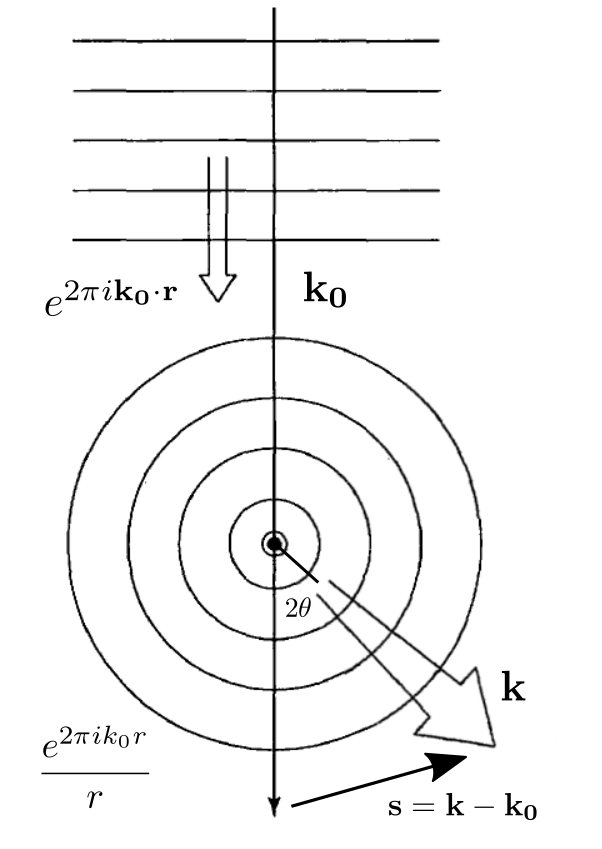
\includegraphics[width=.5\linewidth]{Scattering.png}
	\caption{平面波弹性散射过程的基本描述,参考 \cite{griffiths2016introduction}. }
	\end{figure}
	
	我们介绍晶体分析的基本方法,并将X射线衍射的过程自然推广为电子衍射。\linebreak 晶体由晶胞对叠而成。我们首先考虑单晶,记位于原点的晶胞势场为$\varphi_0(\vb{r})$, 则晶体的势场可表示为:
	\begin{equation}
		\varphi(\vb{r}) = \sum_{l,m,n}
			\varphi_0 \pqty\Big{\vb{r} - (l\vb{a} + m\vb{b} + n\vb{c})}
			= \varphi_0(\vb{r}) \ast \sum_{l,m,n}
			\delta \pqty\Big{\vb{r} - (l\vb{a} + m\vb{b} + n\vb{c})}
	\end{equation}
	其中$(l\vb{a} + m\vb{b} + n\vb{c}),\  l,m,n\in\mbb{Z}$描绘了晶格点阵,而$\ast$表示卷积。对于弹性散射而言,引用电磁波散射的相应结论,设散射所得的次波为
		$\Phi(\vb{s}) \,\frac{e^{2\pi i k_0 r}}{r}$, 
		$\vb{s} = \vb{k} - \vb{k_0}$为散射方向相对原方向的偏离,
	则散射振幅将是势场的傅立叶变换;具体对电子而言,有\footnote{
		参见 \cite{textbook}, p. 207. 
	}:
	\begin{equation}
		\Phi(\vb{s})
		= \frac{2\pi me}{h^2} \fourierf\Bqty{\varphi(\vb{r})}
		= F(\vb{s}) \sum_{h,k,l}
		\delta \pqty\Big{\vb{\vb{s}}
			- (h\vb{a}^\star + k\vb{b}^\star + l\vb{c}^\star)}
	\end{equation}
	这里运用了卷积定理,且此处的傅立叶变换采用了 \cite{textbook} 中的约定\footnote{
		同样参见 \cite{textbook}, p. 207, 即约定
		$ \fourierf\Bqty\big{f(\vb{r})}_{(\vb{s})}
		= \displaystyle\int \dd{\vb{r}}
			f(\vb{r})\,e^{2\pi i \vb{s}\cdot\vb{r}} $.  
	};$F(\vb{s})$是单个晶胞的散射振幅,它包含了系数$\frac{2\pi me}{h^2}$. 
	
	$(h\vb{a}^\star + k\vb{b}^\star + l\vb{c}^\star)$是晶格点阵的傅立叶变换像,它是动量(波矢)空间中的点阵,称为倒易点阵(reciprocal lattice)。这里我们仅考虑立方晶系,则
		$\norm{\vb{a}} = \norm{\vb{b}} = \norm{\vb{c}} = a$为晶格常量,
	$\vb{a},\vb{b},\vb{c}$两两正交,进而有:
	\begin{equation}
		\norm{\vb{a}^\star} = \norm{\vb{b}^\star} = \norm{\vb{c}^\star}
		= \frac{1}{a},\quad
		\textit{$\vb{a}^\star,\vb{b}^\star,\vb{c}^\star$两两正交}
	\end{equation}
	衍射极强出现在$\vb{s} = h\vb{a}^\star + k\vb{b}^\star + l\vb{c}^\star$处,对于立方晶系,此时:
	\begin{equation}
		s = \norm{\vb{s}} = \frac{\sqrt{h^2 + k^2 + l^2}}{a}
	\end{equation}
	
	约定衍射角为$2\theta$, 在小角度近似下,有
		$\sin(2\theta) = \frac{s}{k_0} = s\lambda
		= \frac{\lambda}{a} \sqrt{h^2 + k^2 + l^2}$, 即:
	\begin{equation}
		\sin\theta = \pqty{\frac{\lambda}{a}} \frac{\sqrt{h^2 + k^2 + l^2}}{2}
		\label{eq:DiffEq}
	\end{equation}
	测得衍射极强对应的角$\theta$和相应的德布罗意波长$\lambda$, 即可推算出$a$以及衍射极强对应的指数$(h,k,l)$, 进而得到晶体的结构。
	
	对于多晶而言,其晶胞的取向各异,衍射图样为各取向晶胞的衍射图样之叠加;假定多晶中晶胞各种取向概率均等,将得到各向同性的衍射图像,这正是所谓的德拜环(Debye rings)。
	
	由于薄金属(多晶)样品可以通过沉积法制备,较为简易,我们将首先以电子束透射金属多晶,尝试观察电子衍射产生的德拜环,这将再次验证电子的波动特性。
\section{实验装置}
%	在此部分需要将实验条件交待清楚到别人能重复你的实验结果的程度. 此外,还需表明你已尽了最大努力来提高实验精度和结果的可靠性. 简单的不确定度估计可以在此节给出,复杂一些的可以放到分析讨论部分.\par
%	实验条件不仅是指直接影响实验结果的实验参量,而且还包括影响实验质量和可靠性的因素,如室温、空气湿度、基真空、原材料纯度等.\par
%	作为教学实验报告,此节写详细一点没有坏处.\par
%	成段有叙述,必要才分节。
%%%%%%%%%%%%%%%%%%%%%%%%%%%%%%
	本实验采用透射电子显微镜(Transmission electron microscope, TEM)实现电子的加速及透射成像。本次使用的仪器型号为JEM-200CX, 购置于1981年11月,其结构示意图与实际照片如 \autoref{fig:TEM} 所示。
	
	\begin{figure}[!ht]
	\centering
	\newcommand{\TEMfigHeight}{22\baselineskip}
	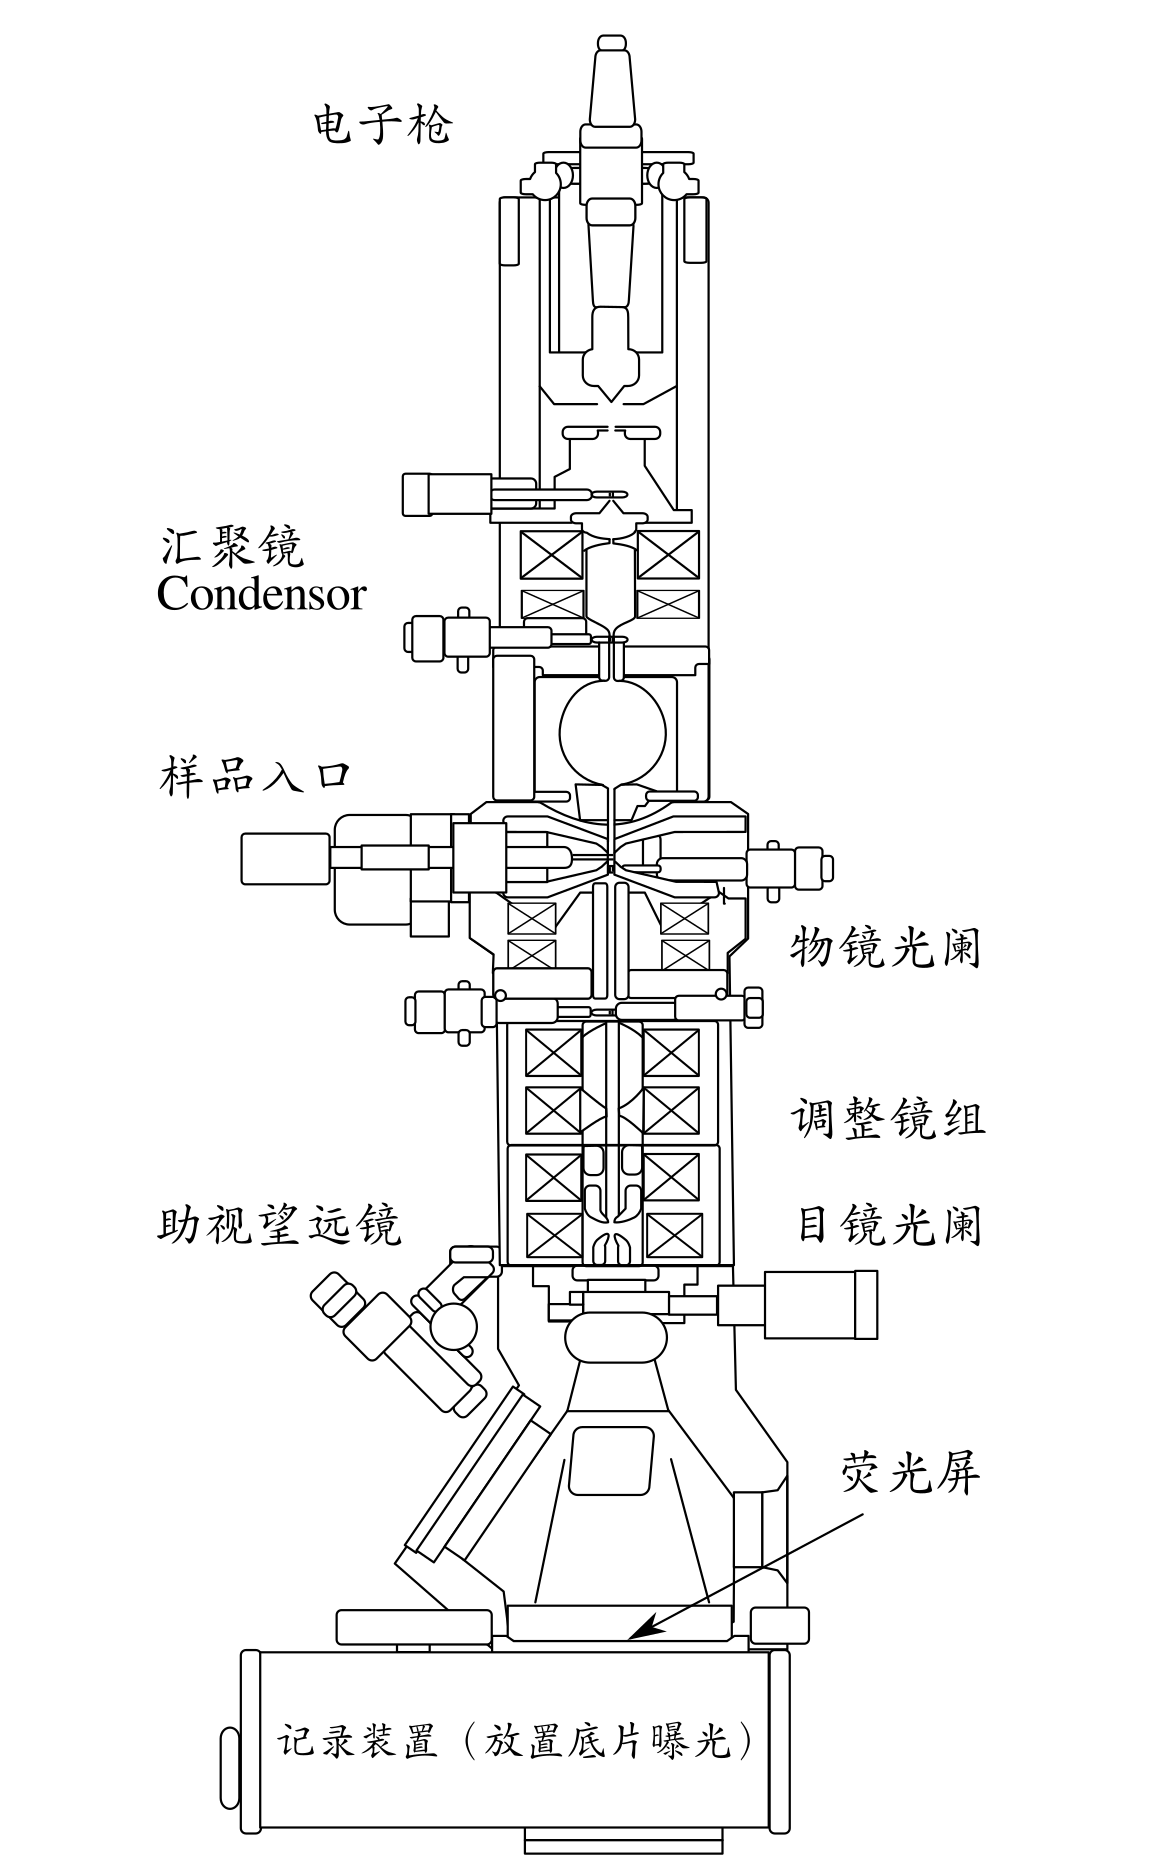
\includegraphics[height=\TEMfigHeight]{Scheme_TEM}\ 
	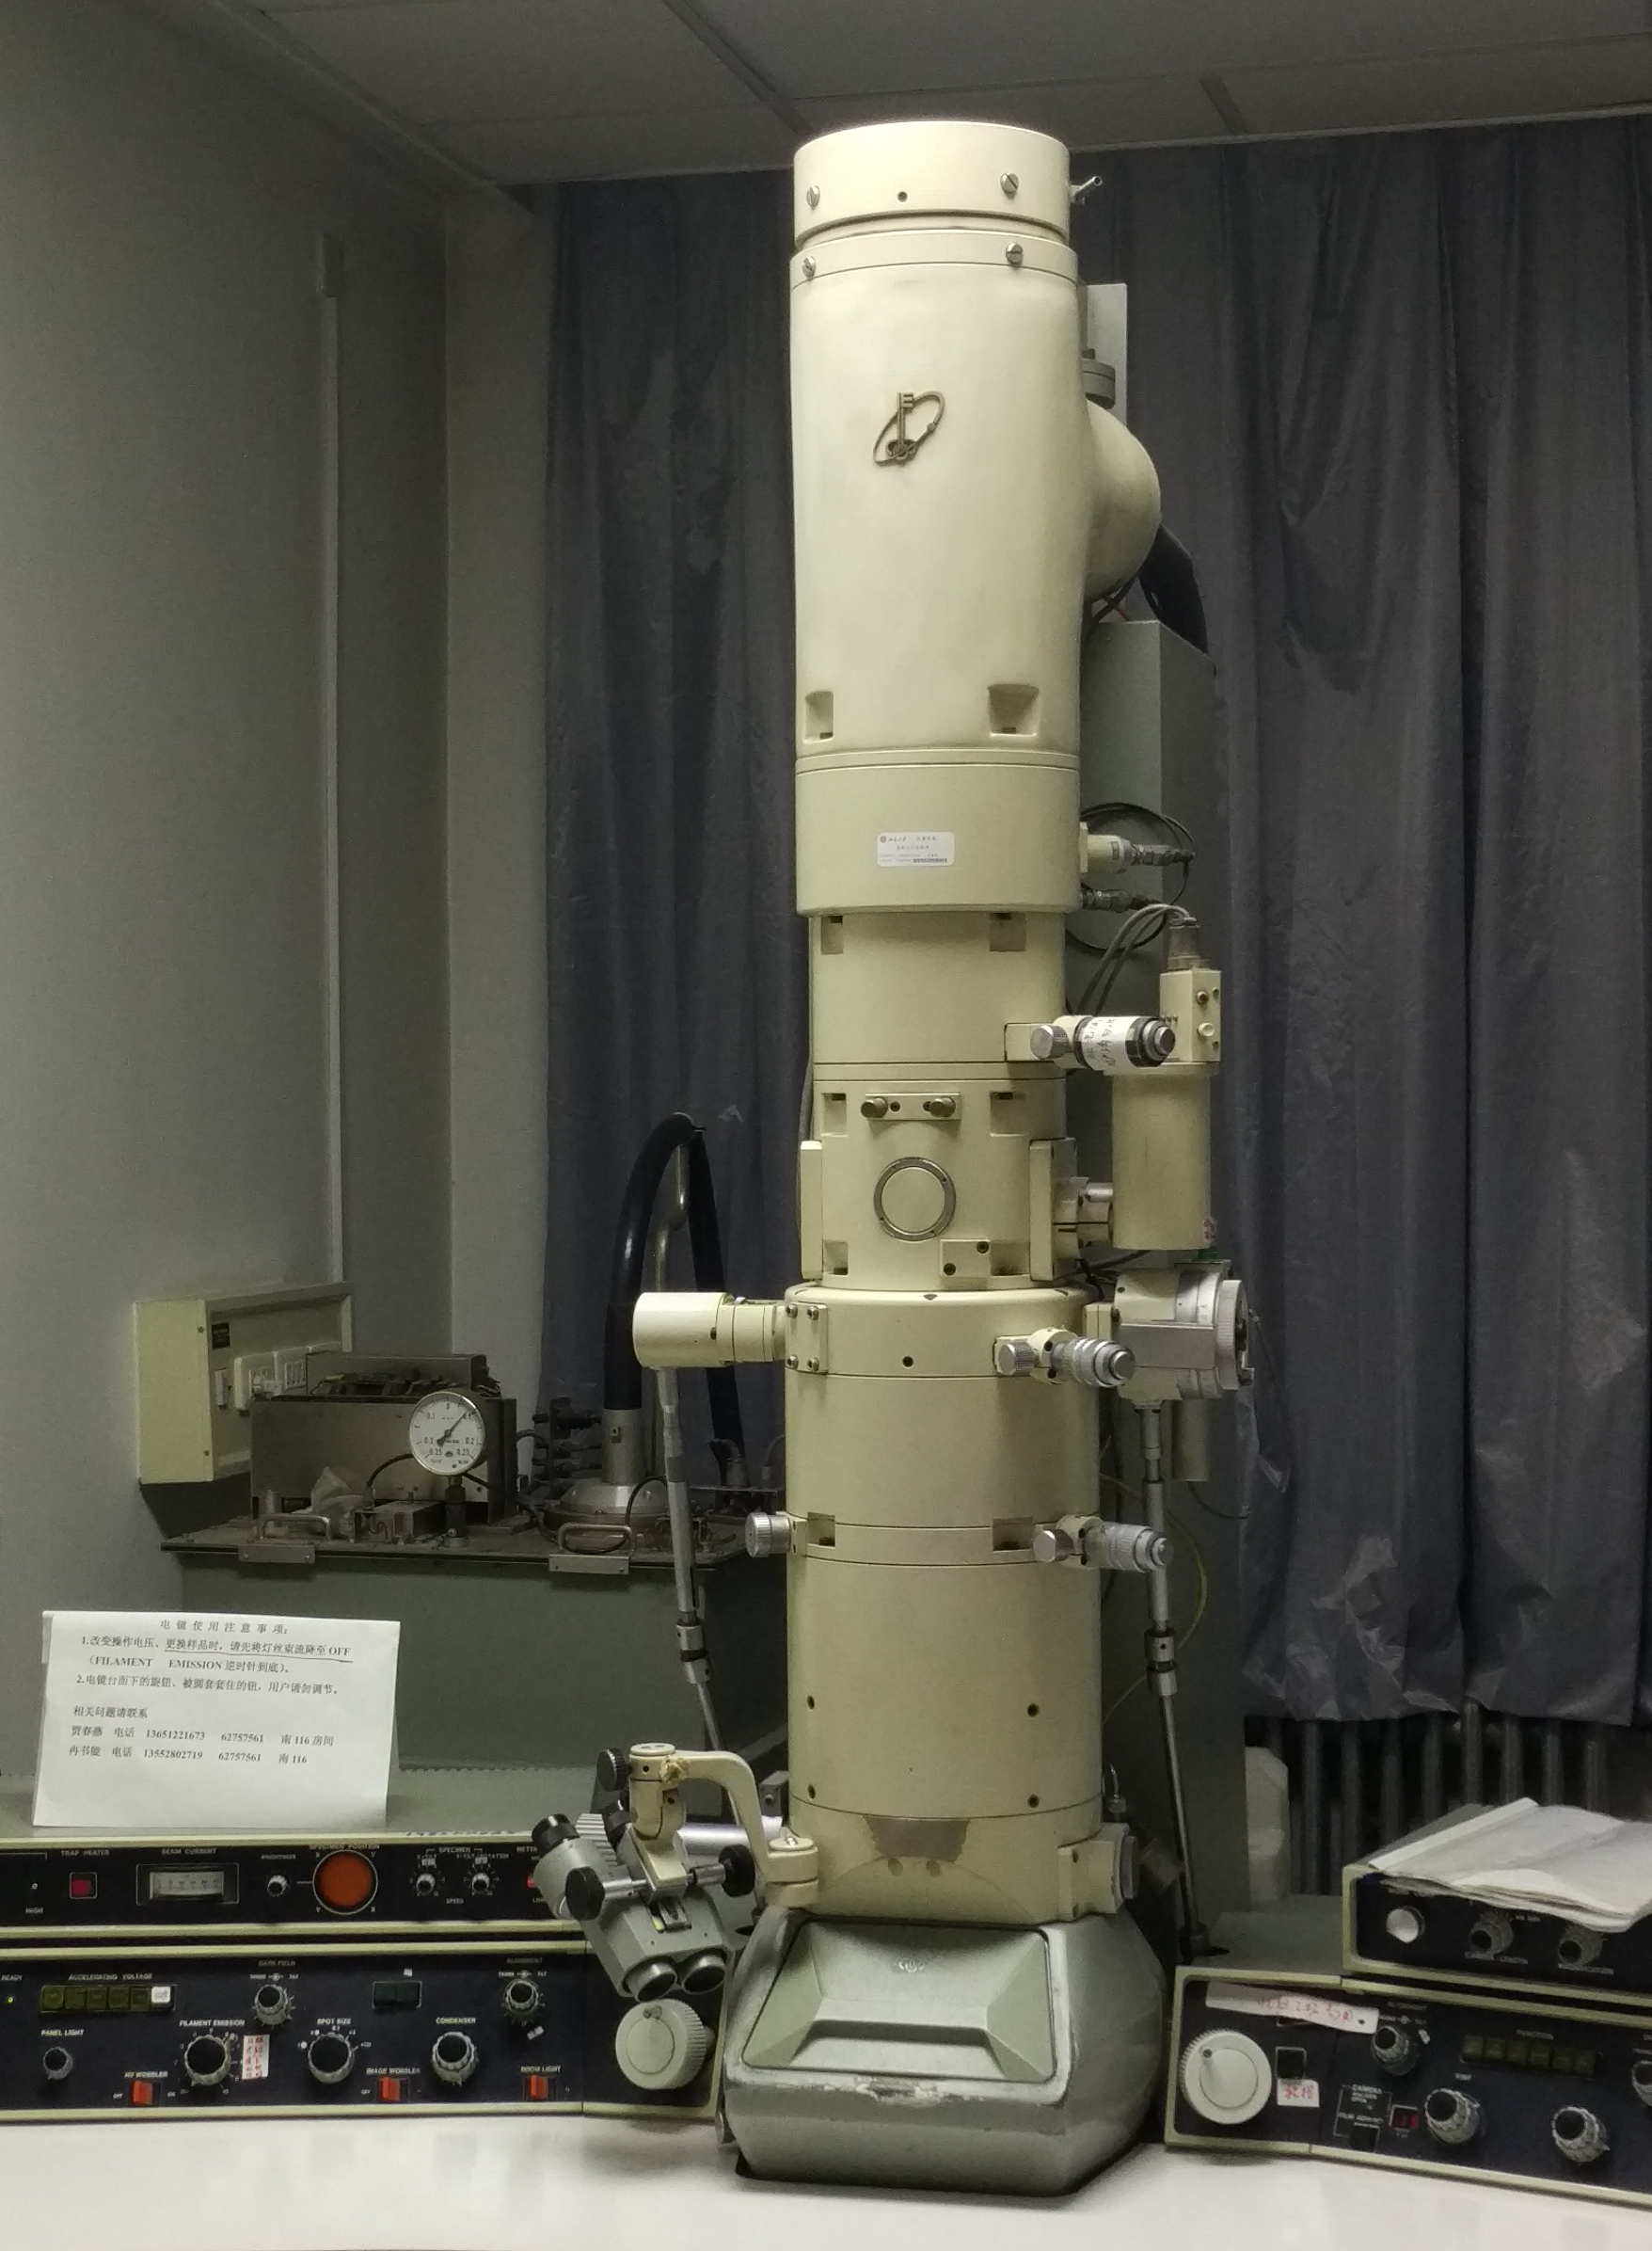
\includegraphics[height=\TEMfigHeight]{RealTEM}
	\caption[透射电子显微镜]{透射电子显微镜\textup{JEM-200CX}, \\
		左为一般的透射电子显微镜之原理示意图\footnote{%
			图像据网络资源修改得到:\par
			\noindent%\fontsize{9pt}{\parskip}%
			\url{https://zh.wikipedia.org/wiki/File:Scheme_TEM_en.svg}%
		},右为实际用仪器的照片。
		\vspace{1ex}}
	\label{fig:TEM}
	\end{figure}
	
	仪器生产的年代早于信息时代,故所有的操作均通过操作控制台上的按键与旋钮完成。然而,电子加速和散射应当在真空中进行,因此仪器通过精妙的设计,几乎实现了电子加速、样品调整、衍射图样记录曝光的自动化。
	
	TEM对电子束流的调整通过\textit{电子透镜}实现。如 \autoref{fig:TEM} 所示,此处大量借用了光学中的术语;这是因为电子透镜对电子束的作用类似于光学透镜对光线的作用,但实际上并非字面上的\textit{镜面}。
	
	使用TEM时,首先保证真空环境;在此基础上,加 160kV 加速电压,调整汇聚系统,使透射电子成清晰的几何光学像;此时TEM处于MAG模式,显示倍率为$100^{\times 1000}$, 在荧光屏上可见样品的表面形貌。事实上,戴维森--革末实验的初衷正是用电子反射构成的几何光学像来研究镍的表面\supercite{davisson1927diffraction}。
	
	上述操作并不依赖电子的波动性。\textit{但若电子确实具有波动性,则会对几何光学像的极限分辨率造成限制。}而且,根据阿贝成像原理,此时若切换成像光圈至透镜的后焦面处,而不是像平面上,则将得到物的\textit{频谱面},即衍射图样。调整TEM至SA~DIFF模式,仪器自动完成上述切换。此时,记控制台上的Camera length参数为$L_0$, 在小角近似下,有几何关系:$\sin(2\theta) = \frac{R}{L_0}$, 即:
	\begin{equation}
		\sin\theta = \frac{R}{2L_0}
		\label{eq:GeoRelation}
	\end{equation}
	其中,$R$为荧光屏上的点相对中心的偏离。这一式给出了荧光屏上的点与相应角$\theta$的对应关系。在此基础上进行实验。
\section{结果与分析}
%	实验结果应尽量以图表的形式给出. 每一个图表都应该是完整的,即阅读图表时可以不必依赖正文.\par
%	依自己意愿,实验结果和对结果的分析讨论既可分为两节也可合在一节.\par
%	\begin{table}[h]
%	\caption{元件恒流大小,为什么要左对齐呢?奇怪。}
%	\small
%	\begin{tabularx}{.6\linewidth}{C{.3} C{1}}
%	\toprule
%	\midrule
%		元件\footnote{%
%			注释一个看看%
%		} & 恒流大小\footnote{%
%			再开一个!哈哈
%		} \\
%	\midrule
%		Pt  &
%			$\SI{1.00005}{\mA}
%				= \SI{100.005}{\mV} / \SI{100}{\ohm} $ \\
%	\midrule
%	\bottomrule
%	\end{tabularx}
%	\label{tab:ExTab}
%	\end{table}
%	
%	每个图一般包含:图名、轴名、轴、刻度、标尺、数据点、曲线、图例、标注和图注等部分. 应尽量让读者不看正文就能基本理解图的含意.\par
%	逐点测量得到的函数关系要同时用表格和图给出. 需要作比较的多条曲线要画在同一图上.\par
%	为避免读者在图表和正文间反复跳跃阅读,在正文中也要对图表作必要的说明.\par
%	
%	对于预料之外的实验结果,必须首先小心证明其可靠性.读者只有在相信你的实验结果时才愿意花时间看你的分析.\par
%	必须用文字归纳整理出正式的实验结果或结论.可信的实验结果是课程报告最重要的内容.作为一个实验物理工作者,分析解释出错并不丢脸,实验结果不被采信则是致命的.\par
%	教学实验的结论往往是预先知道的. 所以,教师更关心的是你的说理过程. 一般说来,单由课内实验的结果不足以能得到明确的结论. 此时,你可以引用他人的研究结果来帮助帮助自己的论证,但必须注明出处. \par
%	确实不能得到明确结论时,可以给出几种可能结论并指出可以再做哪些实验来帮助作进一步的判断.\par
%	总之,分析讨论部分要做到: 论据要valid,论证要reasonable,结论要convincing.\par
%%%%%%%%%%%%%%%%%%%%%%%%%%%%%%
\subsection{多晶衍射的德拜环}
	首先观察多晶银(Ag)样品。按上一节所述准备仪器后,荧光屏上立即可见略微模糊的环状图样。调整$L_0 = \SI{82}{cm}$, 微调聚焦,得到了清晰的图像,如 \autoref{fig:DebyeRings} 所示。
	
	\begin{figure}[!ht]
	\centering
	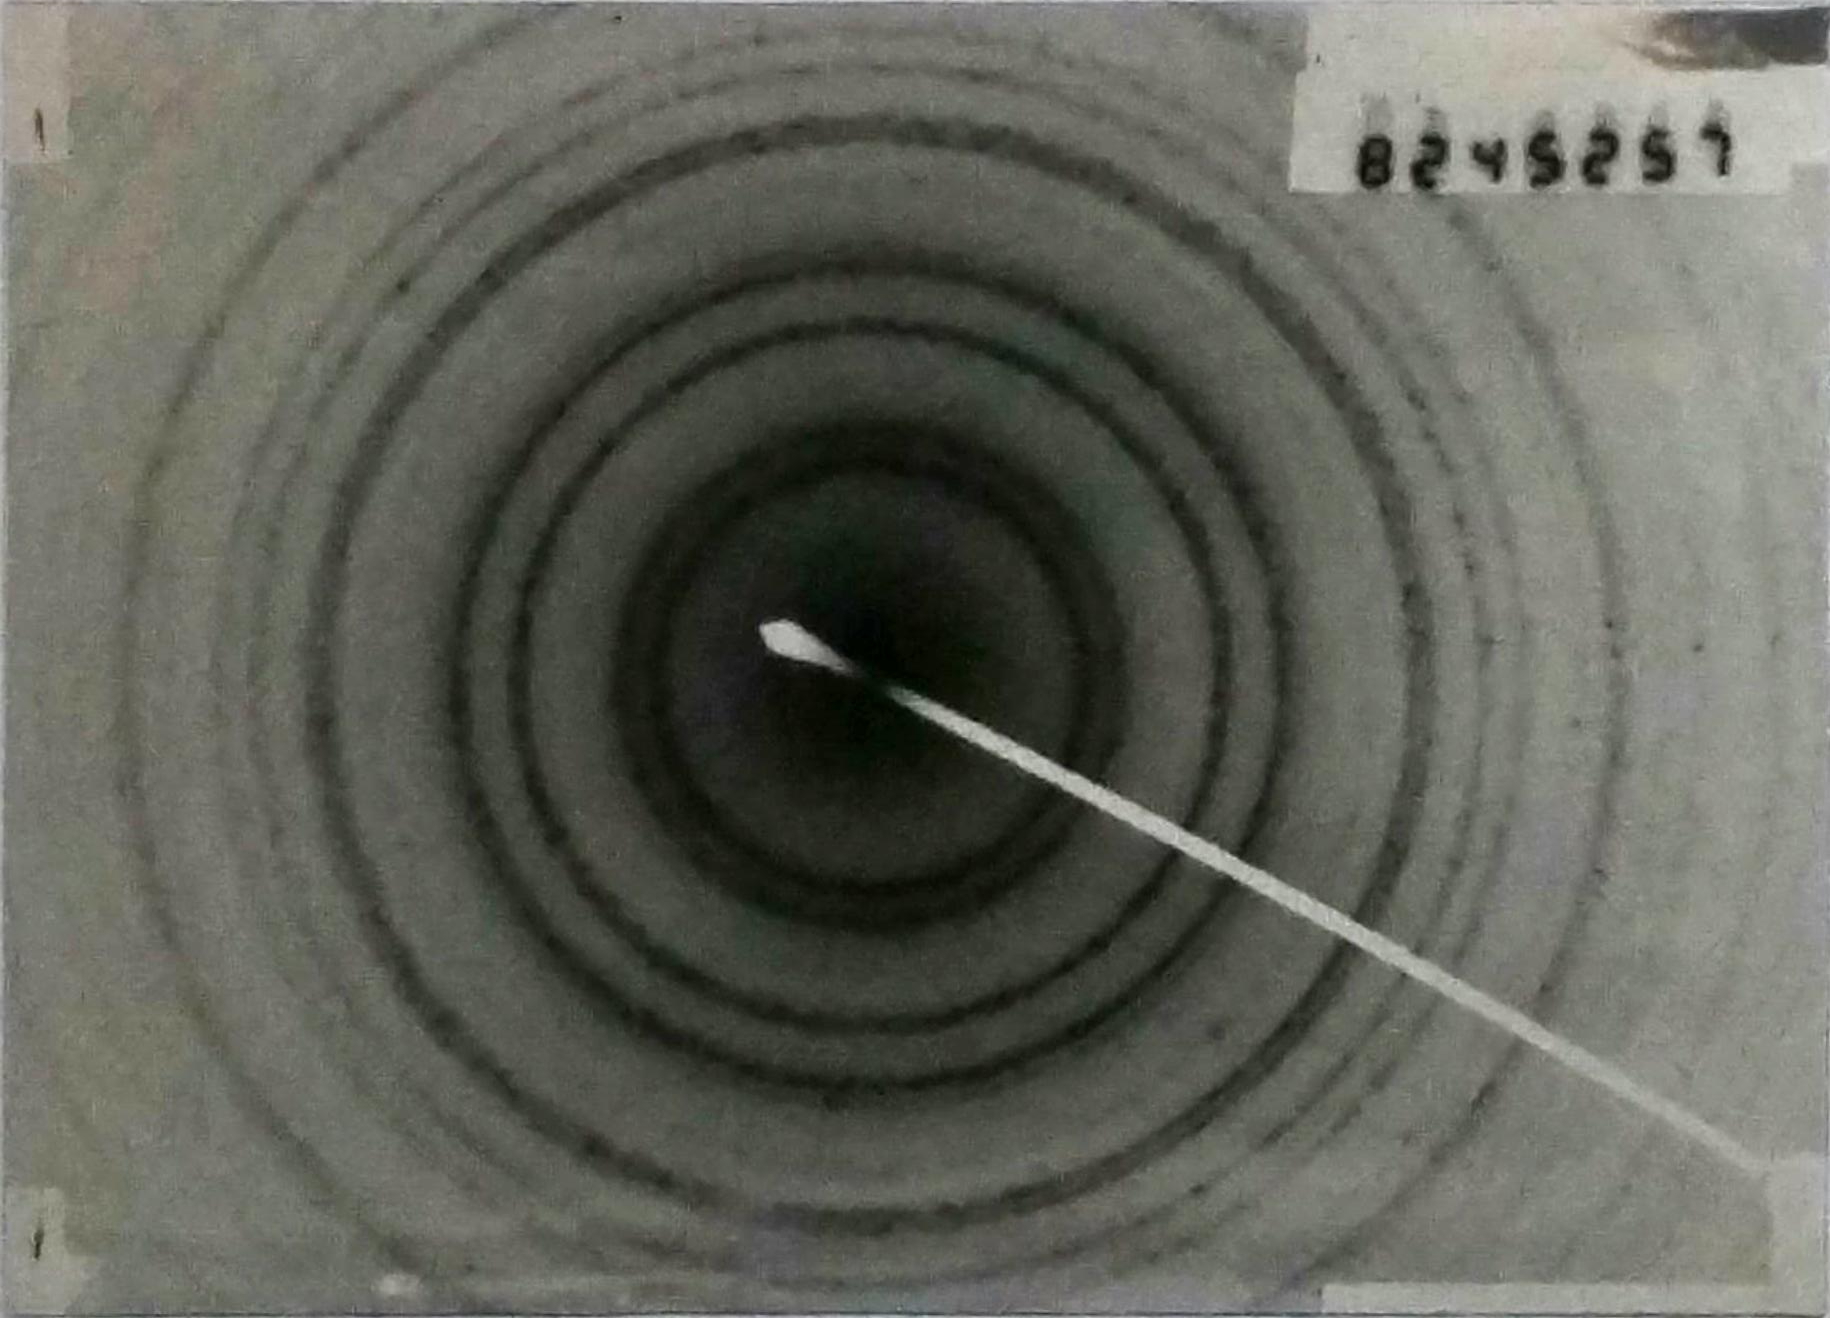
\includegraphics[width=.7\linewidth]{DebyeRings}
	\caption{多晶银(\textup{Ag})的电子衍射图样(德拜环),\\
		(Camera length $L_0 = \SI{82}{cm}$, 
		底片编号\textnumero\,45257\,)}
	\label{fig:DebyeRings}
	\end{figure}
\FloatBarrier
	
	观察图样,其结构与X射线衍射的德拜环完全类似;这便又一次验证了电子的波动性。与最早检验物质波假定的戴维森--革末实验 \cite{davisson1927diffraction} 相比,我们采用了透射电子而非反射电子的方案,这对样品制备有更高的要求。
	
	\newparagraph
	在此基础上,利用晶体学的方法研究衍射图样。对多晶银(Ag)、多晶金(Au)、多晶铜(Cu)重复上述操作,获得相应的德拜环;测量各级衍射环的半径$R$, 利用 \eqref{eq:GeoRelation} 得到相应的$\sin\theta$; 结合 \eqref{eq:DiffEq}, 可以得到关于指数$(h,k,l) \in \mbb{N}$和常量$\pqty{\frac{\lambda}{a}}$的不定方程组。这一方程可以采用 \cite{textbook} 中介绍的指标化方法几何地求解\footnote{%
		参见 \cite{textbook}, p. 195. }。
	
	\begin{table}[!th]
	  \centering
	  \caption{多晶\textup{Ag}衍射环半径$R$及对应的指数$(h,k,l)$, \\
	  $(h,k,l)$利用指标化方法获得,$\Delta R / R$衡量了两组数据的差异。\\
	  “--”表示该衍射环不够清晰,未能记录或比较。}
	    \begin{tabularx}{.7\linewidth}{*4{C{1}}}
	    \toprule\midrule
		    \multicolumn{2}{c}{$R / cm$} &
		    \multirow{2}{*}{\hfil $(h,k,l)$} &
		    \multirow{2}{*}{\hfil $\Delta R / R$} \\
	    \cmidrule{1-2}
		    \textnumero\,45257 & 
		    \textnumero\,45258 &       &  \\
	    \midrule
		    1.04  & 1.02  & 111   & 1.96\% \\
		    1.21  & 1.19  & 200   & 1.68\% \\
		    1.72  & 1.71  & 220   & 0.58\% \\
		    2.00  & 2.01  & 311   & 0.50\% \\
		    2.10  & 2.16  & 222   & 2.86\% \\
		    2.42  & --    & 400   & -- \\
		    2.65  & --    & 331   & -- \\
		    2.73  & --    & 420   & -- \\
		    2.98  & 2.98  & 422   & 0.00\% \\
		    3.15  & 3.17  & 333/511 & 0.63\% \\
	    \midrule\bottomrule
	    \end{tabularx}%
	  \label{tab:AgData}%
	\end{table}%
	
	对多晶Ag, 我们拍摄了两张衍射图样,并分别由不同的两人进行测算和分析,结果如 \autoref{tab:AgData} 所示。比较可知,在距离$R$的测算上,两人的结果有不超过 3\% 的差异;以此作为测量结果不确定度的一个估计。利用指标化方法,相应地给出:
	\begin{equation}
	\pqty{\frac{\lambda}{a}} =
	\Bigg\lbrace\begin{aligned}
		& \num{7.40e-3},\quad \textnumero\,45257,\\
		& \num{7.38e-3},\quad \textnumero\,45258,
	\end{aligned}\qquad
	\pqty{\frac{\lambda}{a}}_{\textup{Ag}} = \num{7.39(2)e-3}
	\end{equation}
	注意到,这两个结果的差异只有 0.3\%, 远小于前面估计的 3\%, 这是因为$(h,k,l)\in\mbb{N}$的约束条件实际上对误差有一定的控制作用;或者说,$(h,k,l)\in\mbb{N}$相当于在求解的过程中有一步\textit{取整}的运算,这导致最终结果对度数造成的误差并不敏感。\vspace{2ex}
\pagebreak[3]
	
	根据$(h,k,l)$可能的取值,查表\footnote{%
		同样参见 \cite{textbook}, p. 195, 表 5-0-2. }可知,Ag具有面心立方晶胞。
	类似地,对多晶Au, Cu的衍射图样进行分析,结果综合于 \autoref{tab:AuCuData} 和 \autoref{tab:aMetal}. 
	\begin{table}[!ht]
	  \caption{多晶\textup{Au, Cu}衍射环半径$R$及对应的指数$(h,k,l)$, \\
	  $(h,k,l)$利用指标化方法获得。}
	\begin{tabularx}{.65\linewidth}{C{1}C{1}|C{1}C{1}}
	\toprule\midrule
		\multicolumn{2}{c|}{Au, \textnumero\,45259} &
		\multicolumn{2}{c}{Cu, \textnumero\,45260}\\ 
	\midrule
		$R / cm$ & $(h,k,l)$ &
		$R / cm$ & $(h,k,l)$ \\
	\midrule
		1.02 & 111 & 1.17 & 111 \\ 
		1.18 & 200 & 1.32 & 200 \\ 
		1.66 & 220 & 1.90 & 220 \\ 
		1.93 & 311 & 2.20 & 311 \\ 
		2.04 & 222 & 2.91 & 331 \\ 
		2.37 & 400 & 3.27 & 422 \\ 
		2.56 & 331 & 3.49 & 333/511 \\ 
		2.65 & 420 &  &  \\ 
		2.89 & 422 &  &  \\ 
		3.07 & 333/511 &  &  \\ 
	\midrule\bottomrule
	\end{tabularx}
	\label{tab:AuCuData}
	\end{table}
	
	\begin{table}[!ht]
	  \caption{多晶\textup{Ag, Au, Cu}的$\pqty{\frac{\lambda}{a}}$和$a$测定值,\\[.5ex]
	  通过指标化方法得到,其中$a$为晶格常量,$\lambda$为入射波长。\\
	  $a_{\textup{Au}}$为标准参考值,以之定标得到其余的$a$值。}
	\begin{tabularx}{.6\linewidth}{*4{C{1}}}
	\toprule\midrule
		金属多晶 & Ag & Au & Cu \\
	\midrule
		$\pqty{\frac{\lambda}{a}} / \times\num{e3}$ &
		7.39 & 7.22 & 8.20 \\
	\midrule
		$a / \si{\angstrom}$ & 3.98 & 4.08 & 3.59 \\
	\midrule\bottomrule
	\end{tabularx}
	\label{tab:aMetal}
	\end{table}
	
	由于电子波长$\lambda$以及长度$L_0$的具体值不甚确定,我们取$a_{\textup{Au}} = \SI{4.0786}{\angstrom}$对结果进行定标,得到其余金属的$a$值。如果相信$L_0 = \SI{82}{\cm}$是充分精确的,我们将得到,
	\begin{equation}
		\lambda \approx \SI{.029}{\angstrom}
	\end{equation}
	由 \eqref{eq:deBroglieLambda} 可得$\lambda \approx \SI{.031}{\angstrom}$, 两者基本一致。
	
	参考 \cite{PhysRev.25.753}, 利用X射线衍射得到的晶格常量如 \autoref{tab:aMetalX} 所示。比较可见,电子衍射与X射线衍射测定的结果基本一致,但存在一定差异。首先,我们使用的标准值$a_{\textup{Au}}$源自于 \cite{textbook}, 其值大小本身就与 \autoref{tab:aMetalX} 中的参考值不同;此外,由于样品晶格实际上是三维点阵,衍射图样实际上也具有三维结构,这导致像具有一定的\textit{景深};根据傅立叶变换的倒易特性,样品越薄,沿样品厚度方向的衍射展宽越大\footnote{%
		详细讨论参见 \cite{textbook}, p.\numrange{211}{212}. 
		}。因此,所拍摄的底片可能并没有恰好对焦,这也将给测定结果造成一定的误差。
	
	\begin{table}[!ht]
	  \caption{【参考】利用X射线衍射测定的金属多晶之晶格常量$a$,\\
	  	数据来源于 \cite{PhysRev.25.753}. }
	\begin{tabularx}{.6\linewidth}{*4{C{1}}}
	\toprule\midrule
		金属多晶 & Ag & Au & Cu \\
	\midrule
		$a / \si{\angstrom}$ & 4.079 & 4.065 & 3.597 \\
	\midrule\bottomrule
	\end{tabularx}
	\label{tab:aMetalX}
	\vspace{-3ex}
	\end{table}
\subsection{单晶衍射的劳厄斑}
	\begin{figure}[!ht]
	\centering
	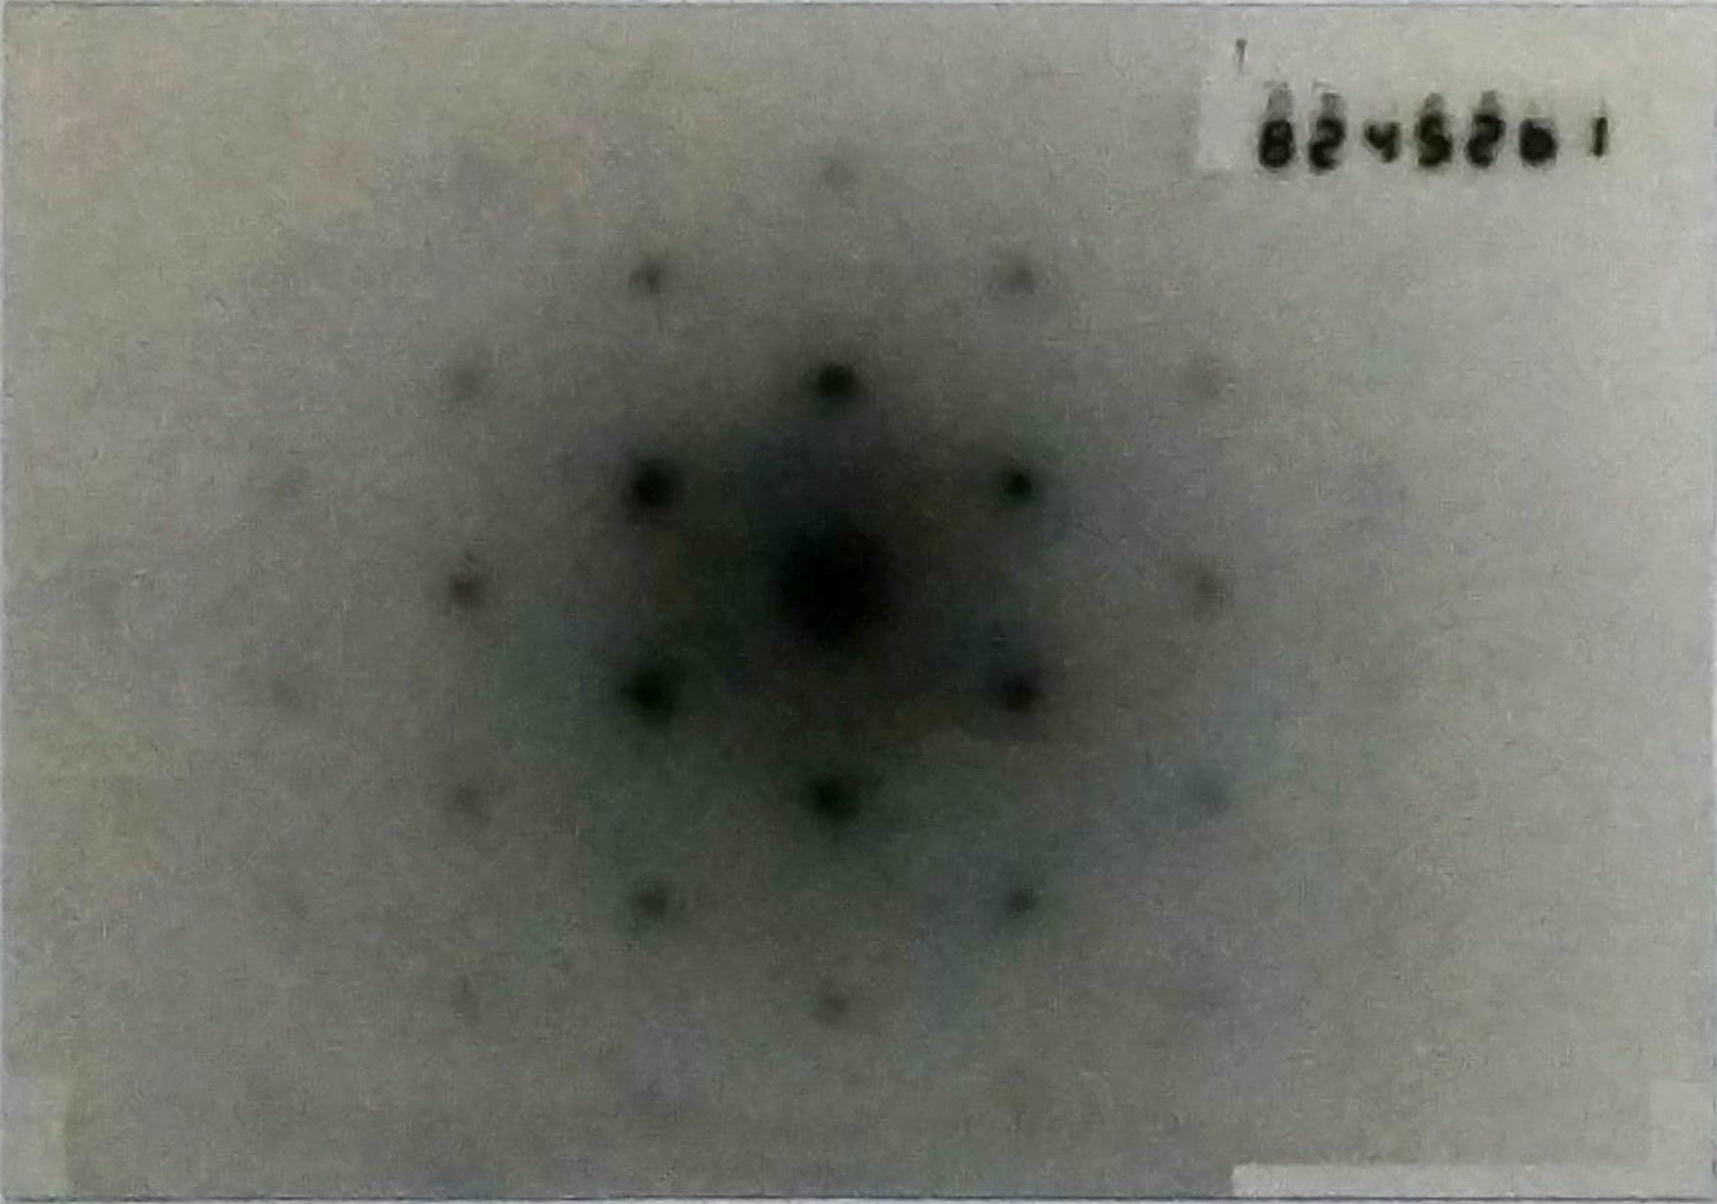
\includegraphics[width=.7\linewidth]{LaueSpots}
	\caption{单晶硅(Si)的电子衍射图样(劳厄斑),\\
		(Camera length $L_0 = \SI{82}{cm}$, 
		底片编号\textnumero\,45261\,)}
	\label{fig:LaueRings}
	\end{figure}
	
	进一步,取单晶硅(Si)为样品观察衍射图样。选取样品边缘可透射区域进行观察,在衍射模式下,立即可见点阵状的衍射斑。微调样品的倾角,得到旋转对称的衍射图样;相邻3点均构成正三角形,如 \autoref{fig:LaueRings} 所示。
	
	曝光获得底片,测定任意两衍射斑点的间距,得到常量:
	\begin{equation}
		R_0 = \SI{1.12(5)}{\cm}
	\end{equation}
	利用衍射图样的对称性,可以无需测量,通过计算得到任意级别衍射斑到中心的距离$R$. 事实上,如 \autoref{fig:SiLattice} 所示,有:
	\begin{equation}
	\begin{aligned}
		\frac{R}{R_0}
		&= m \sqrt{\pqty{\frac{\sqrt{3}}{2}}^2
			+ \pqty{n + \frac{1}{2}}^2} \\
		&= m \sqrt{n^2 + n + 1},\quad
		n = 0,1,2,\dots,\quad
		m = 1,2,3,\dots
	\end{aligned}
	\end{equation}
	\begin{figure}[!ht]
	\centering
	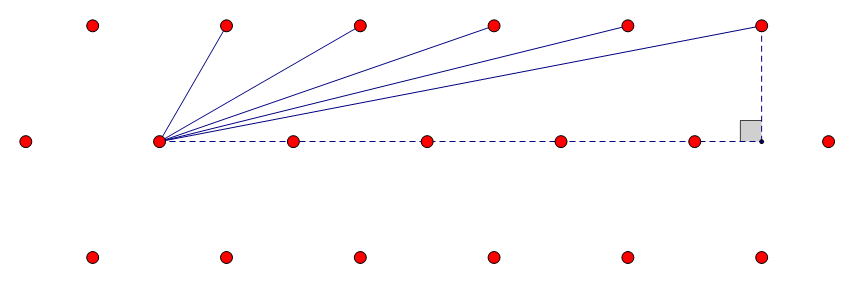
\includegraphics[width=.6\linewidth]{SiLattice.png}
	\caption{单晶硅的劳厄斑示意图,\\
		各级衍射斑点偏离中心的距离如图所示。}
	\label{fig:SiLattice}
	\end{figure}
\FloatBarrier
	
	由对称性,可依次得到相应斑点对应的指标;类似可得,单晶Si也是面心立方结构,且:
	\begin{equation}
		a = \SI{5.4(2)}{\angstrom}
	\end{equation}
	比较参考值\supercite{CODATAVa61:online} $a = \SI{5.431}{\angstrom}$, 可见两者基本吻合。同样,可能的差异或许来源于景深问题,需要进一步实验加以证实。
\section{结论}
%	首先要给出实验结果,然后再给出由实验结果分析得到的结果和结论.此部分给出的内容要比摘要中的全面,用词要更准确.\par
	本次实验利用透射电子的方案,再一次证实了电子的波动特性;在此基础上,成功地将X射线衍射晶体学的方法应用在了电子衍射的图像分析中,验证了TEM物质分析的可行性。
\section{致谢}
%	此部分感谢同组人...和对实验和报告有帮助的人.
	感谢我的合作伙伴曹睿枭同学,他的工作是不可或缺的;感谢耐心的指导老师对我们的巨大帮助。
\section{参考文献}
\bibliographystyle{../BibStyle/gbt-7714-2015-numerical}
\bibliography{../BibStyle/Textbook,bib/Ref}
\clearpage
\end{document}
